\documentclass[12pt]{beamer}
\usepackage[utf8]{inputenc}
\usepackage[T1]{fontenc}
\usepackage{lmodern}
\usepackage[spanish]{babel}
\usepackage{amsmath}
\usepackage{amsfonts}
\usepackage{amssymb}
\usepackage{graphicx}
\usepackage{hyperref}
\usepackage{multicol}
\usepackage{dirtree}
\usepackage{etoolbox} % to reduce spacing in bearmers toc
\usetheme[block=fill]{metropolis}

\begin{document}
	\author{Fernando Oleo Blanco \\ fernando.oleo@alu.comillas.edu \hfill 	\href{https://github.com/Irvise/Documents}{github.com/Irvise/Documents}}
	\title{Introducción a Linux}
	%\subtitle{}
	%\logo{}
	\institute{ICAI - LinuxEC}
	\date{\today}
	%\subject{}
	%\setbeamercovered{transparent}
	\setbeamertemplate{navigation symbols}{}
	\setbeamertemplate{footline}[page number]
\begin{frame}[plain]
	\maketitle
\end{frame}

\begin{frame}[allowframebreaks]{Índice}
%\vfill
\tableofcontents
%\clearpage
\end{frame}

\section{Historia}

\begin{frame}[plain]
	\begin{figure}
		\centering
		\vspace*{10px}
		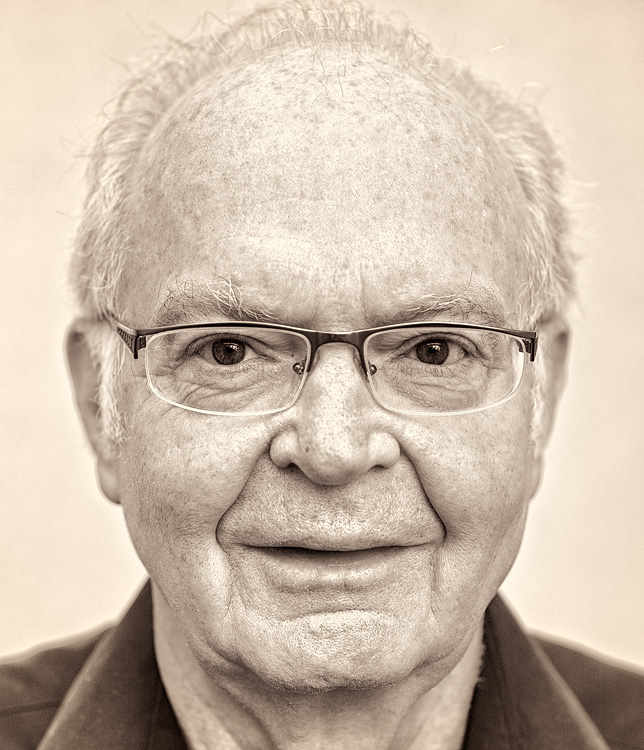
\includegraphics[height=0.75\linewidth]{Donald-Knuth-Stanford-Computer-Science}
		\caption{Donald Ervin Knuth. Creador de \TeX}
		\label{fig:donald-knuth-stanford-computer-science}
	\end{figure}
\end{frame}

\begin{frame}{Un pequeño cuento}
\small
\begin{block}{¿Quién es Knuth?}
	Americano. Profesor de Stanford, ya retirado. Matemático, físico, informático y teólogo. Actualmente escribe la serie de libros \texttt{The Art of Computer Programming,} precursora del nacimiento de \TeX. Considerado uno de los padres de la informática moderna
\end{block}

\begin{block}{\TeX}
	Después de crear el segundo volumen y empezar el tercero se dio cuenta que la tipografía carecía calidad. Buscó soluciones y decidió estudiar tipografía para crearse su propio sistema. \TeX es el entorno de programación, \LaTeX\ es \TeX\ y unos paquetes para agilizar su escritura
\end{block}

	\textit{"Si una herramienta que uso la utilizan muchas personas, seguramente pensaría que estoy haciendo algo mal"}

\end{frame}

\section{Instalación y recursos}

\begin{frame}{Instalación}

\begin{block}{TexStudio, IDE}
	$\bullet$ \href{http://www.texstudio.org/}{\textbf{\TeX Studio:}} Download $\rightarrow$ busca tu plataforma. Instálalo como solo tú sabes
\end{block}

\begin{block}{\LaTeXe}
	$\bullet$ \href{https://www.latex-project.org/get/}{\textbf{"Compilador"}} \\
	Windows: usad o Mik\TeX\ o Texlive. Texlive es el tradicional\\
	Mac: instalad Mac\TeX\ y listo
	Linux: buscad \texttt{texlive} en buestra distribución
\end{block}
\begin{block}{Recursos on-line}
	Accesibles desde el link anterior. Es una buena idea tener una copia en la nube. Recomiendo \href{https://www.overleaf.com/}{Overleaf,} recientemente fusionado con Share\LaTeX
\end{block}
\end{frame}

\begin{frame}{Recursos recomendados}
\begin{block}{Lectura}
	$\bullet$ \href{https://tobi.oetiker.ch/lshort/lshort.pdf}{\textit{The not so Short Introduction to \LaTeX}} por Tobias Oetiker \\
	$\bullet$ \href{https://en.wikibooks.org/wiki/LaTeX}{\textit{\LaTeX\ Wikibook:}} Libro escrito por y para Wikipedia. El 99\% de vuestras dudas tienen solución aquí \\
	$\bullet$ \href{http://osl.ugr.es/CTAN/info/Math_into_LaTeX-4/Short_Course.pdf}{\textit{More Math Into \LaTeX}} por George Grätzner (esta es una buena muestra)
\end{block}
\begin{block}{Internet}
	$\bullet$ Cualquier servicio con plantillas (\href{http://www.latextemplates.com/}{\textbf{Latextemplates}} por ejemplo) \\
	$\bullet$ \href{https://www.tug.org/begin.html}{\textbf{Tug:}} Centro de recursos \textit{oficiales} \\
	$\bullet$ Foros (\href{https://www.overleaf.com/learn}{\underline{\textbf{Overleaf-learn}}}), "puntos de información", etc \\
	$\bullet$ Google
\end{block}

\end{frame}

\section{Comparativa con Word}

\begin{frame}[t]{Diferencias notables}
	\begin{columns}[t]
		\begin{column}{0.4\textwidth}
			Microsoft Word
			\begin{itemize}
				\item Intuitivo, fácil de usar
				\item Ya conocido
				\item Imágines, tablas, etc se hacen solas \\
				\hrulefill
				\item ¿Bibliografía?
				\item ¿Índice?
				\item ¿Referencias?
			\end{itemize}
		\end{column}
		\begin{column}{0.55\textwidth}
			\LaTeX
			\begin{itemize}
				\item Complicado, tedioso
				\item Con un error, ya nada funciona
				\item Escribirlo todo manualmente...\\
				\hrulefill
				\item Estructura automática
				\item Texto de calidad sin esfuerzo
				\item No da problemas las dos semanas antes de la entrega
			\end{itemize}
		\end{column}
	\end{columns}
\end{frame}

\section{Estructura del documento}

\begin{frame}{Estructura de archivos}
	Estructura de archivos
	\begin{columns}
		\begin{column}{0.4\textwidth}
			\dirtree{%
				.1 /. 
				.2 main.tex. 
				.2 bliblio.bib. 
				.2 \dots. 
				.2 Cap1. 
				.3 cap1.tex. 
				.3 img.png. 
				.3 pdf.pdf. 
				.3 \dots. 
				.2 Cap2. 
				.3 \dots. 
			}
		\end{column}
		\begin{column}{0.6\textwidth}
			En \LaTeX\ podemos, y se recomienda, dividir nuestro archivo en partes pequeñas y en carpetas. Esto permite estructurar mucho mejor el documento, mantener los archivos ordenados, y trabajar con textos menores.
		\end{column}
	\end{columns}
\end{frame}

\subsection{\texttt{\ documentclass y preámbulo}}

\begin{frame}[fragile]{Estructura general de los comandos}
	\begin{block}{Comando tradicional}
		Comienzan con $\textbackslash$, seguido del comando. Si este comando recibe algún argumento (o algunos), estos van entre llaves. Si reciben opciones, van entre corchetes antes del argumento. Ejemplos: \\
		\verb|\hrulefill| $\rightarrow$ \hrulefill \\
		\verb|\textit{Hola}| $\rightarrow$ \textit{Hola} \\
		\verb|\textcolor{blue}{azul}| $\rightarrow$ \textcolor{blue}{azul}
	\end{block}
	\begin{block}{Entornos}
		Como comandos normales, pero cuya función es más extensa y compleja; tienen la estructura \verb|\begin{entorno}[opciones]{argumento}| \verb| content... | 
	\verb|\end{frame}|
	\end{block}
\end{frame}

\begin{frame}{Comienzo de nuestro documento}
	$\bullet$ \textbf{\texttt{\ documentclass}}
	\begin{block}{}
		\textbf{Nuestra primera línea.} Define la naturaleza de nuestro documento.
	\end{block}
\end{frame}

\subsection{Manejo del texto}
asdf
\subsubsection{Entornos comunes}

\subsection{Referencias y bibliografía}

\section{Escritura científica}

\section{Resumen y otros recursos}

\end{document}